\documentclass[a4paper, 14pt]{extarticle}%тип документа

%Русский язык
\usepackage[T2A]{fontenc} %кодировка
\usepackage[utf8]{inputenc} %кодировка исходного кода
\usepackage[english,russian]{babel} %локализация и переносы

%отступы 
\usepackage[left=2cm,right=2cm,top=2cm,bottom=3cm,bindingoffset=0cm]{geometry}

%Вставка картинок
\usepackage{graphicx}
\usepackage{wrapfig, caption}
\graphicspath{}
\DeclareGraphicsExtensions{.pdf,.png,.jpg, .jpeg}
\newcommand\ECaption[1]{%
     \captionsetup{font=footnotesize}%
     \caption{#1}}

%Таблицы
\usepackage[table,xcdraw]{xcolor}
\usepackage{booktabs}

%Графики
\usepackage{pgfplots}
\pgfplotsset{compat=1.9}
\usepackage{float}

%Математика
\usepackage{amsmath, amsfonts, amssymb, amsthm, mathtools}

%Заголовок
\author{Подлесный Артём \\ группа 827}
\title{Работа 8.1 \\ Определение постоянных Стефана-Больцмана и Планка из анализа теплового излучения накаленного тела}

\begin{document}
\maketitle

\section*{Экспериментальная установка}

\begin{figure}[h]
\begin{center}
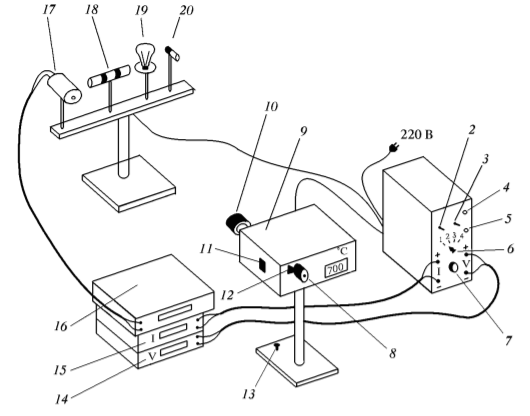
\includegraphics[width=0.7\textwidth]{ust}
\end{center}
\ECaption{Схема установки для исследования закона излучения АЧТ и серых тел. Исследуются 4 образца, пронумерованные с 17 по 20: модель АЧТ, трубка с кольцами из разных материалов, лампа наливания и неоновая лампочка.  }
\end{figure}

С помощью пирометра измеряется яркостная температура тела -- температура, при которой абсолютно черное тело (АЧТ) излучает с той же спектральной испускательной способностью что и исследуемое тело, при той же длине волны. 

Измерение производится с помощью пирометра с пропадающей нитью. Пирометр показывает яркостную температуру нити, и для начала работы было необходимо проверить, что это действительно температура АЧТ. С помощью модели 1 образца, это было проделано с помощью термопары и формулы баланса потребляемой и излучаемой энергии:
\[W = \sigma (T^4-T_0^4).\]
Для температуры в 20$^{\circ} C$, полученная температура АЧТ совпадало с температурой пирометра, так что в дальнейшем им действительно можно пользоваться.

\section*{Измерение яркостной температуры тел}

В этом пункте работы исследуется второй образец. Он представляет из себя керамическую трубку с двумя надетыми на неё кольцами из разных материалов. Трубка была нагрета до яркостной температуры в 917$^{\circ} C$. Одновременно с этим можно было измерить яркостную температуру колец, качественно, лишь примерно из-за сложности в получении результатов. Они составили:
\[T_{\text{ярк}} = 818\parallel 812^{\circ}C, \text{ для 1 и 2 колец соответственно.}\]

Разница в температурах объясняется различным коэффициентом излучения ($\varepsilon_T$) для разных материалов. Закон Стефана-Больцмана для серых тел выражается формулой
\begin{equation}
R_T = \varepsilon_T \sigma T^4.
\end{equation}
Тогда для 2 разных материалов коэффициенты будут разные, а значит при одинаковой температуре они излучают по-разному, а значит яркостная температура будет различаться.

Эксперимент понятен, но в данной установке, из-за наличия дневного света, практически невозможно увидеть цвет излучения на белой трубке и блестящих кольцах, не то что увидеть разницу в их яркости. Так что установку я бы серьезно переработал, иначе весь эксперимент просто подгоняется на ранее известный результат, никакой беспристрасной проверки просто не происходит. Ситуацию мог бы улучшить красный фильтр на 6500 A, но при такой температуре свечения через фильтр практически не видно, так что на нашей установке его нельзя было использовать.

\section*{Проверка закона Стефана-Больцмана}

На этом этапе работы проверяется закон Стефана-Больцмана для серого тела -- вольфрамовой нити 3 образца.  С помощью пирометра измеряется яркостная температура нити $T_{\text{ярк}}$, c шагом в 100 градусов, в зависимости от мощности, потребляемой лампой, которая оценивается с помощью напряжения, показываемого вольтметром, и силы тока на амперметре. Далее с помощью графика зависимости температуры вольфрама $T(T_{\text{ярк}})$, рис. 2(а), получаем зависимость $T(W)$, представленная на таблице 1.

\begin{figure}[h!]
\begin{minipage}[h]{0.5\linewidth}
\center{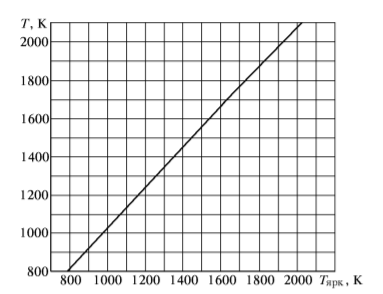
\includegraphics[width=1\linewidth]{ust1} \\ (a)}
\end{minipage}
\hfill
\begin{minipage}[h]{0.5\linewidth}
\center{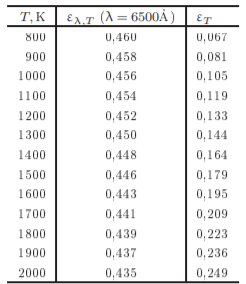
\includegraphics[width=1\linewidth]{ust2} \\ (б)}
\end{minipage}
\ECaption{a) График зависимости температуры вольфрама от его яркостной температуры $T(T_{\text{ярк}})$. б) Таблица коэффициентов излучения вольфрама в зависимости от температуры.}
\end{figure}


По полученным данным можно построить график в логарифмическом масштабе, используя следующую формулу:
\begin{equation}
\text{ln}W = \text{ln}\varepsilon_T B + n\text{ln}T,
\end{equation}
где $B = \sigma \cdot S$ -- эффективная площадь излучающей поверхности. Естественно эти значения зависят от температуры нити - нить излучает по всей поверхности при температуре более 1700К, однако в логарифмическом масштабе эти изменения можно не учитывать.


Из графика (рис.3) получаем значение для степени в законе Стефана-Больцмана (1):
\[n = 4.1 \pm 0.1.\]




\begin{table}[!h]
\begin{center}
\begin{tabular}{|c|c|c|c|c|}
\hline
\rowcolor[HTML]{9698ED} 
$T_{\text{ярк}}$, C & $U$, B & $I$, A & $T$, K & $W$, Вт \\ \hline
1000                & 1.955  & 0.51   & 1443   & 0.997   \\ \hline
\rowcolor[HTML]{9698ED} 
1100                & 2.348  & 0.55   & 1551   & 1.291   \\ \hline
1200                & 2.718  & 0.585  & 1659   & 1.590   \\ \hline
\rowcolor[HTML]{9698ED} 
1300                & 3.268  & 0.629  & 1767   & 2.056   \\ \hline
1400                & 4.016  & 0.696  & 1875   & 2.795   \\ \hline
\rowcolor[HTML]{9698ED} 
1500                & 5.011  & 0.774  & 1984   & 3.879   \\ \hline
1600                & 6.256  & 0.864  & 2092   & 5.405   \\ \hline
\rowcolor[HTML]{9698ED} 
1700                & 6.233  & 0.863  & 2200   & 5.379   \\ \hline
1600                & 5.243  & 0.792  & 2092   & 4.152   \\ \hline
\rowcolor[HTML]{9698ED} 
1500                & 4.729  & 0.752  & 1984   & 3.556   \\ \hline
1800                & 7.199  & 0.928  & 2308   & 6.681   \\ \hline
\rowcolor[HTML]{9698ED} 
1900                & 8.218  & 0.92   & 2416   & 7.561   \\ \hline
1900                & 8.718  & 1.024  & 2416   & 8.927   \\ \hline
\end{tabular}
\ECaption{Экспериментальные данные зависимости $T(W)$. Здесь есть несколько значений для одной и той же температуры, что связано с тем, что на глаз определять, когда "исчезает" нить пирометра -- очень сложно, и порой носит рандомный характер. При построении графика будет понятно, какие результаты более достоверные. Но с учетом того, каким образом дали зависимость $T(T_{\text{ярк}})$ понятно отношение к точности в этой работе.}
\end{center}
\end{table}




\begin{figure}[H]
\begin{center}
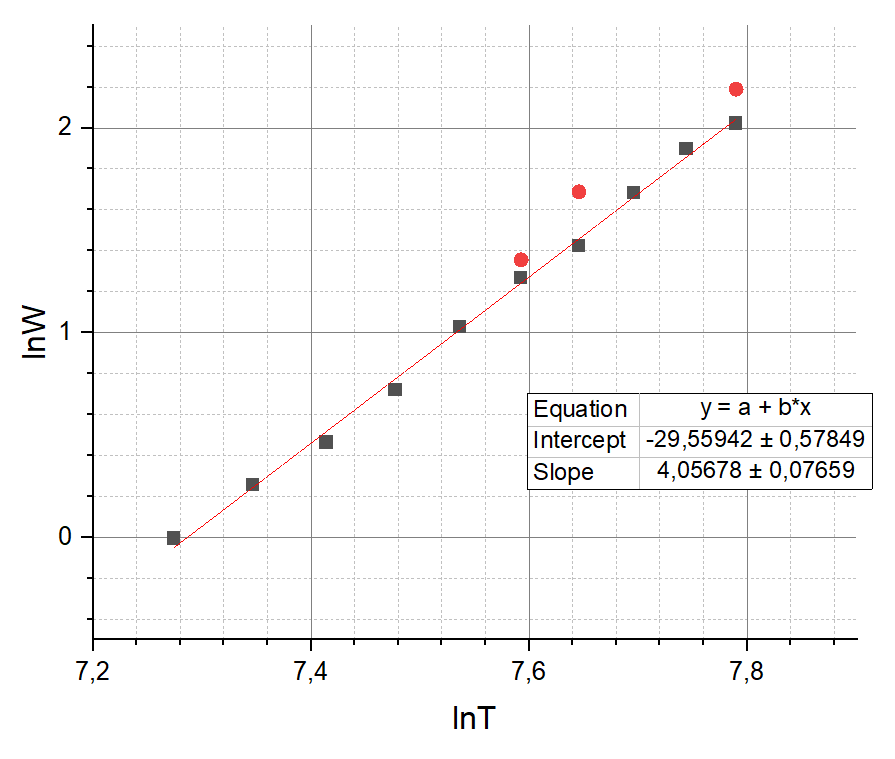
\includegraphics[width=0.73\textwidth]{gr1}
\ECaption{Закон Стефана-Больцмана в логарифмическом масштабе (2). Точки, которые были перемеряны при выполнении эксперимента, отмечены на графике красным. Видно, что они действительно являются недостоверными.}
\end{center}
\end{figure}



\subsection*{Определения постоянных Стефана-Больцмана и Планка}

При температуре нити больше 1700К вся нить равномерно накалена, а значит можно количественно определить величину постоянной Стефана-Больцмана:
\begin{equation}
\sigma = \frac{W}{\varepsilon_T S T^4},
\end{equation}
где $S = 0.36 \text{ см}^2$. По полученным значениям была оценена постоянная Планка по следующей формуле:
\begin{equation}
h = \sqrt[3]{\frac{2\pi^5 k_{\text{Б}}^4}{15c^2\sigma}}.
\end{equation}
Результаты оценки представлены на таблице 2.

\begin{table}[h!]
\begin{center}
\begin{tabular}{|c|c|c|c|c|}
\hline
\rowcolor[HTML]{9698ED} 
$T$, K & $\varepsilon_T$ & $W$, Вт & $\sigma$, Вт/см$^2\cdot K^4$ & $h$, кг$\cdot$м$^2\cdot c^{-1}\cdot 10^34$ \\ \hline
1767   & 0.22            & 2.06    & 5.27E-12                     & 6.79                                       \\ \hline
\rowcolor[HTML]{9698ED} 
1875   & 0.23            & 2.80    & 5.07E-12                     & 6.88                                       \\ \hline
1984   & 0.25            & 3.56    & 4.68E-12                     & 7.07                                       \\ \hline
\rowcolor[HTML]{9698ED} 
2092   & 0.26            & 4.15    & 4.03E-12                     & 7.42                                       \\ \hline
2200   & 0.28            & 5.38    & 3.93E-12                     & 7.49                                       \\ \hline
\rowcolor[HTML]{9698ED} 
2308   & 0.29            & 6.68    & 3.72E-12                     & 7.62                                       \\ \hline
2416   & 0.31            & 7.56    & 3.26E-12                     & 7.97                                       \\ \hline
\end{tabular}
\ECaption{Постоянные Стефана-Больцмана и Планка, измеренные при разных температурах для равномерно накаленной нити.}
\end{center}
\end{table}

Видно, что значения для постоянных различаются при разной температуре. Табличные значения постоянных:
\[\sigma = 5.67 \times 10^{-12}\text{ } \frac{\text{Вт}}{\text{см}^2\text{К}^4},\]
\[h = 6.626 \times 10^{-34} \text{ кг}\cdot\text{м}^2\cdot c^{-1}.\]
Как видно, результаты совпадают с табличными значениями только по порядку. Это закономерный результат, о причинах расхождения будет сказано в выводе.
\newpage

\subsection*{Измерение яркостной температуры неоновой лампочки}

Последний этап работы проводится на 4 образце - неоновой лампочке. Её яркостная температура была оценена как 953$^{\circ}$. При этом ее реальная температура была комнатной. Этот факт можно объяснить тем, что неон является принципиально другим источником света - газоразрядным.

 Атомы инертного газа возбуждаются под действием поданного напряжения, но находиться в этом состоянии долго не могут. Поэтому через короткий промежуток времени, исчисляемый миллионными долями секунды, электрон с резонансного уровня возвращается в нейтральное положение.
 
При обратном переходе электрона с резонансного уровня в нейтральное положение происходит излучение энергии в виде определённой порции света, кванта света - фотона. 

\section*{Вывод}

В работе исследовался закон Стефана-Больцмана, и он подтвердился с достаточно хорошей сходимостью и достоверностью. Однако количественные оценки оказались крайне неточными, и сильно различались при разной температуре. Это можно объяснить несколькими факторами. Первый -- теоретический, состоит в особенности вольфрама в виде селиктивности излучения -- на коротких волнах интенсивность видимого излучения существенно больше, чем следует из закона для серого тела. В частности поэтому экспериментальные значения постоянных ухудшались по мере увеличения температуры.

Однако в данной работе более существенным является факт общей неточности постановки эксперимента. Очень сложно получить четкий момент исчезновения нити, и результаты будут сильно искажены особенностью цветовосприятия глаза, так что реальную погрешность метода даже сложно оценить. При этом данные для обработки даются в виде странного графика, где нет точных значений коэффициентов прямой (рис.2 a), и таблицы с определенными коэффициентами излучения, не теми, которые измеряются в самой работе. В таких условиях не получается провести ничего кроме оценочной работы с большими погрешностями, что я и сделал.


















\end{document}